% Created 2010-12-19 Sun 22:09
\documentclass[11pt]{article}
\usepackage[utf8]{inputenc}
\usepackage[T1]{fontenc}
\usepackage{fixltx2e}
\usepackage{graphicx}
\usepackage{longtable}
\usepackage{float}
\usepackage{wrapfig}
\usepackage{soul}
\usepackage{t1enc}
\usepackage{textcomp}
\usepackage{marvosym}
\usepackage{wasysym}
\usepackage{latexsym}
\usepackage{amssymb}
\usepackage{hyperref}
\tolerance=1000
\providecommand{\alert}[1]{\textbf{#1}}

\title{AS-0.3301 Project Documentation: Tower Defense}
\author{Joel Pitkänen <joel.pitkanen@tkk.fi> (82156A),\\ Joonas Nissinen <joonas.nissinen@tkk.fi> (84362C),\\ Ilari T. Nieminen <ilari.nieminen@tkk.fi> (60628W)}
\date{19 December 2010}

\begin{document}

\maketitle

\setcounter{tocdepth}{3}
\tableofcontents
\vspace*{1cm}

\section{Instructions for compiling and use}
\label{sec-1}

% \begin{verbatim}
%  In this chapter you must tell which platform(s) and operating system(s) your program supports.
%  How it can be compiled (and installed) ie. which tools are needed to compile the program and which commands to use.
% \end{verbatim}

The game currently works only on Linux. On Windows, Clanlib misbehaves in interesting ways.

Running:

You need to have ClanLib 2.2.5 (or newer) installed (the version
provided for the course is ok). You also need to have Boost
installed. The program comes with a Makefile, which is located in the
src-directory. To compile, run make in this directory. To run the
program, run the resulting ``td''.

\subsection{How to play the game}
\label{sec-1_1}

You will first see a login screen. You can add a player with the
chosen name by ticking the ``create player'' checkbox. You can protect
your username by giving it a password. Try not to forget your
username/password combination, as otherwise you will need to check it
from the user database file.

After you have chosen the ``New game'' option, you can choose the level
you want to play. You can only choose levels which you have reached.

Defend the exit from enemy hordes by building defensive towers which
will smite them. You may modify the route your enemies take by
building the towers in your enemies' path, but the universe prevents
you from building towers so that you would be able to block your
enemies' progress. The game screen is shown in Figure
\ref{fig:game}. The bar in the lower part of the screen shows the
available towers, their prices. The player's health is shown as a
green bar. Money and score are also shown. When the player has beaten
a wave on enemies, the countdown to the next wave will begin.

You will lose if 20 enemies reach the exit. You will win if you
survive all the waves. If you win, you can proceed to the next
level. Currently, there are three levels.

\begin{figure}[ht!]
\centering
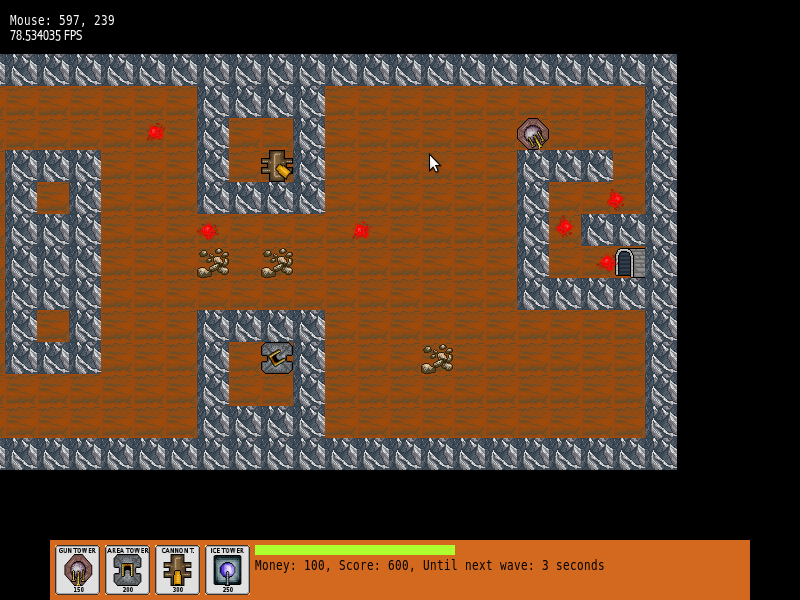
\includegraphics[width=\textwidth]{screenshot.png}
\caption{A screenshot of the game}
\label{fig:game}
\end{figure}


\subsection{Controls}
\label{sec-1_2}

Scroll around the map using the mouse and the right mouse
button. Build towers by selecting the tower you want to build from the
bar in the bottom of the screen, or you can use the shortcuts (number
keys). You can upgrade or sell your towers by clicking on them. By
pressing Q-key, you can see the range of your towers. Pressing ESC-key
brings you back to the menu. For cheaters, there is K-key which will
kill every enemy in game; however, this is only enabled if DEBUG is
true.

\subsection{Mobs and Towers}

There are basically two different types of enemies in the game. Normal
ones and spawners. Normal monsters have different properties, but
simply walk towards the exit. Spawners also walk towards the exit, but
while doing so, they spawn more enemies in their path.

There are four towers in the game:
\begin{description}
\item[GunTower] A basic tower, which damages a single enemy and has a high rate of fire.
\item[CannonTower] A variant of the GunTower, with a larger range and
  damage, but a lower rate of fire.
\item[AreaTower] Tower which causes a small amount of damage to all
  enemies in its range.
\item[IceTower] A variant of the AreaTower which also slows down the
  enemies in range. It also causes a small amount of damage over a
  large period of time.

\end{description}

% \begin{verbatim}
%  You must also tell what your program does and how it can be used. You must also add some
%  example of program runs (example inputs and outputs and/or screenshots or something like that).
%  
%  Add here the manual of your program.
%  
%  This part is important. If the assistant can not understand how to compile and/or use your program by
%  reading these instructions, your project will most propably be failed.
% \end{verbatim}

\section{Program architechture}
\label{sec-2}

The general class structure of the game is shown in \ref{fig:class}.

\begin{figure}
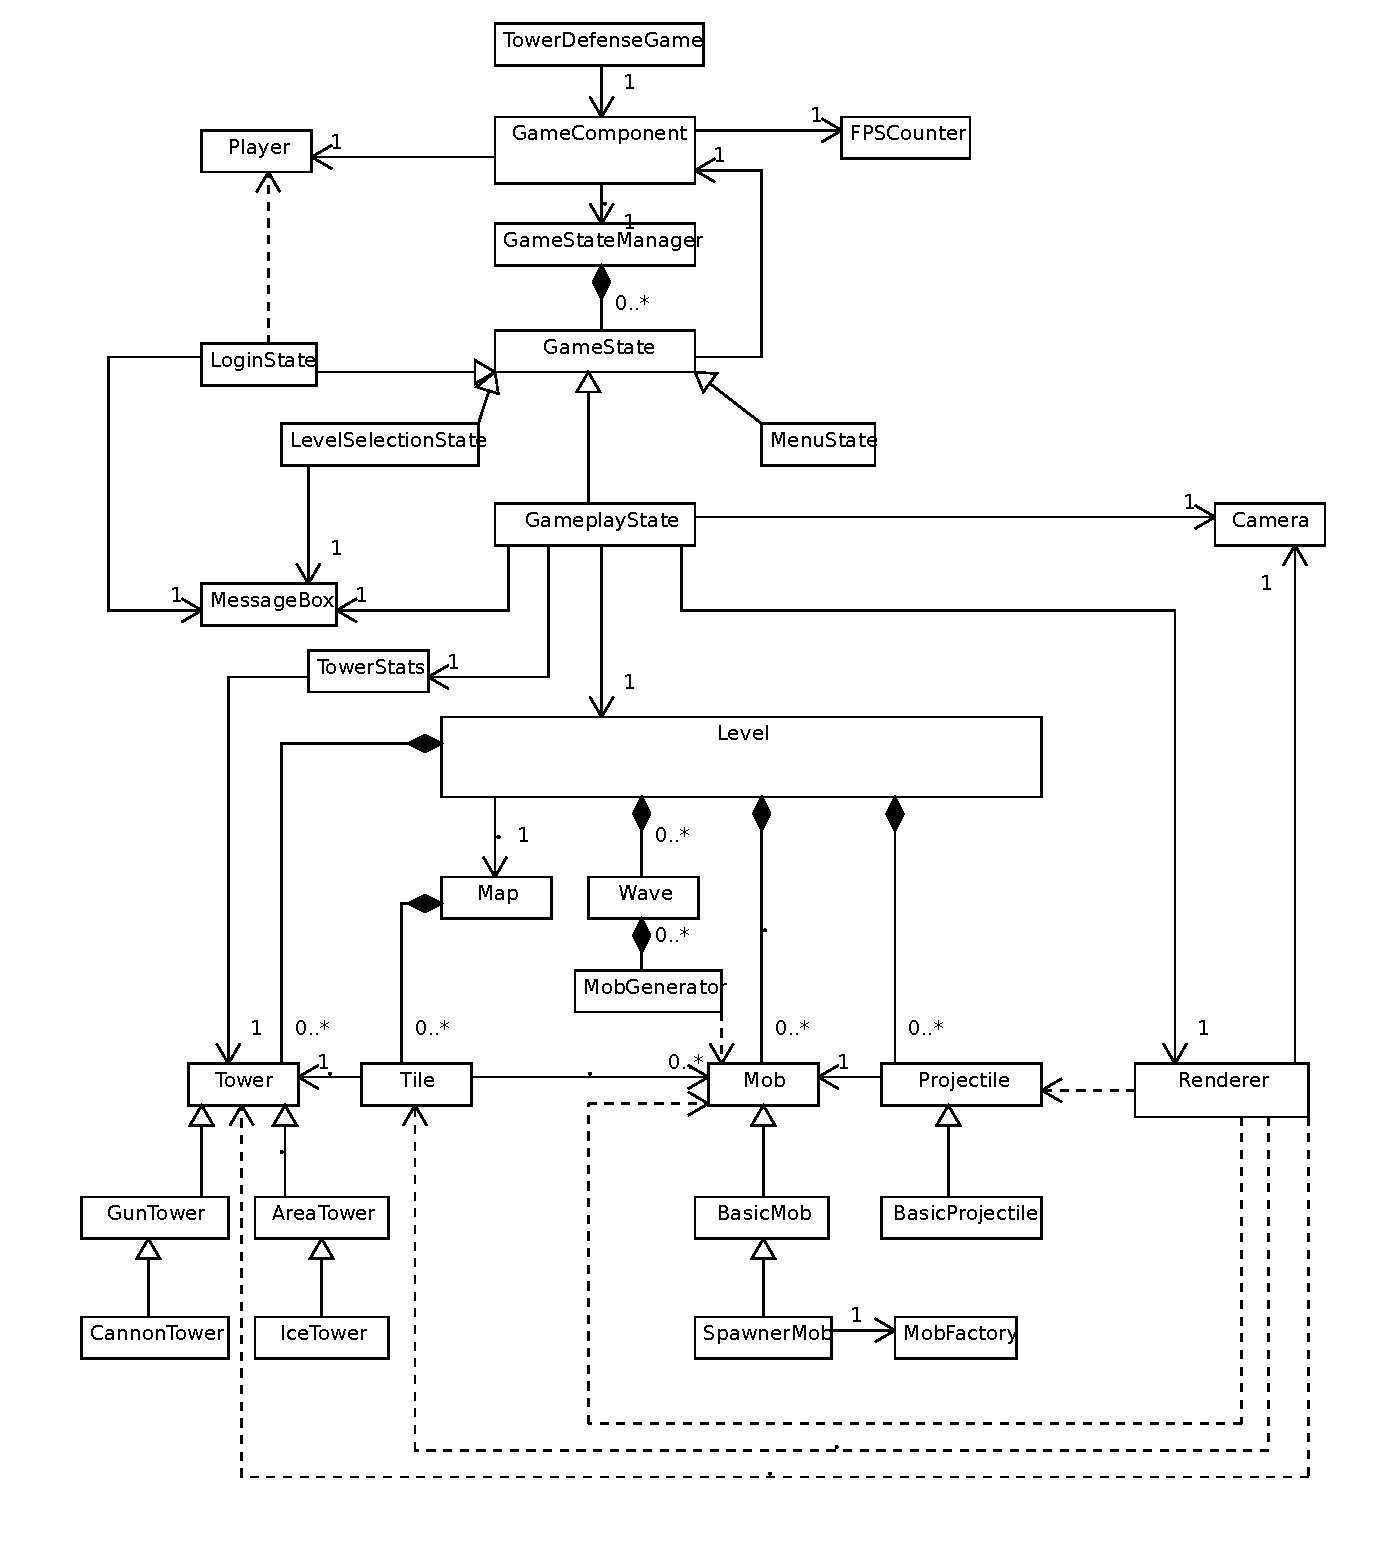
\includegraphics[width=\textwidth]{classdiagram.pdf}
\caption{Class diagram for the game}
\label{fig:class}
\end{figure}

The program consists of different states, which are placed in a stack
and managed by the GameStateManager, which calls the update-function
of the topmost state.

Primary state is the gameplay state, which is responsible for the user
interface for the actual game. Drawing and updating the game state are
done separately.

The actual game entities such as Mob, Tower, Projectile are tied to a
particular Level, which handles most of the game itself.

The particular class division was natural, even though the
dependencies between the classes were not completely shown in the
plan. The basic idea has remained constant, however. The state-based
window handling makes it easy to separate the different parts of the
game. The actual game part is a pretty typical setup, where the game
is updated a fixed number of steps every second.

% \begin{verbatim}
%  In this chapter you must describe the main architechture of your program. You must draw clear diagrams
%  of your program structure. You don't need to go in to the details, but this chapter should give the reader
%  the idea of the architechture of your program. You must also tell, why you decided to use the architechture you used.
% \end{verbatim}
 
\section{Data structures and algorithms}
\label{sec-3}


% \begin{verbatim}
%  In this chapter you must describe the data structures and algorithms used in your program. Dont't put
%  your code here, but describe the data structures and algorithms using natural language (you can also add pictures).
% \end{verbatim}

Most entities, such as mobs and towers are stored in lists. This makes
it easy to process all elements in a sequential manner and also makes
it possible to quickly remove elements from the middle of the list.

For non-instantaneous damage, there is a damage queue, which is
implemented as a priority queue.
 
The routes for enemies are done by calculating the distances from the
exit to all the reachable tiles and keeping track of the direction one
should go to when on the particular tile by going through the tiles in
a breadth-first order. The directions are only updated for the tiles
which are currently reachable from the exit, so an enemy that gets
``stuck'' will simply follow the earlier directions and pass through a
tower.

Many problems were solved in a naïve way, leaving opportunities for
further optimization in case it becomes necessary.
\section{Known bugs}
\label{sec-4}
\subsection*{Bugs and "features"}
\label{sec-4_1}

\begin{itemize}
\item More of a known feature: The maps are not checked strictly
  beforehands and invalid information in a map (for example, wave
  using an entrance not present in the map) will throw an error when
  the map is loaded for use and will cause the game to crash.
\item Projectiles don't behave like one would expect. They are
  currently just a visual aid to show which enemy the tower is
  shooting at. Sometimes the projectile will miss its target, which
  causes flickering in the projectile graphics.
\item The database is not initialized if missing.
\item Using valgrind to get rid of all problems is a bit more
  difficult, as even a barebones Clanlib program will have errors
  valgrind will catch.

\end{itemize}
\subsection*{What could have been done better}
\label{sec-4_2}

\begin{itemize}
\item A more generic way of upgrading the towers. A less manual way of
  inputting the changes if they affect just the numerical properties
  of the tower and not the functionality. The tower information could
  mainly reside in a configurable XML file.
\item Adding new tower types to the game requires a few too many
    steps. Also, there should have been a Tower factory class to hide
    some of the messy details from the interface itself.
\item Pathfinding: Diagonal movement would look better on open maps,
    also the enemies could actually move in a even more optimal manner
    (calculating straight-line paths)
\item The Level class should be split into several classes. (For
    example, pathfinding could be extracted)
\item Targeting is done in a naïve manner: all the enemies are searched
    through, even though getting a list of tiles which are in range
    would not be difficult to do. Going through these in the order of
    distance to the exit would in practice make targeting much faster,
    now it is linear to the number of monsters. With these numbers of
    monsters on the screen, this optimization did not become
    necessary.
  \item The wave handling is done in an extremely convoluted way; it
    should be cleaned up and the logic should be made clear.
  \item For ease of use, the login screen could have had a list of
    players in the database.
  \item The map checking could be more strict, and the maps should be
    checked on startup to avoid errors later in the game.
\item Many changes, especially towards the end were ``kludges''; something
    that could have been done better, but the amount of work for a
    quick fix was lower than a better fix. (Though this is apparently
    rather common in the game industry)
  \item MobGenerator and MobFactory serve partially the same function;
    this should be reflected in the relation.
  \item Variable and method naming is not completely
    consistent. Coding style questions should have been written down
    in the beginning.
  \item Sounds could have been implemented.
  \item The ``kill'' command doesn't actually necessary kill all
    enemies, it just causes a lot of damage.
\end{itemize}


% \begin{verbatim}
%  In this chapter you must tell all known bugs in your code. You must also tell what could have been done better.
%  
%  If the assistant finds bug(s) in your code that you haven't mentioned, it is very bad thing and your points will be
%  decreased. And if your code segfaults, it is even worse and your points will be decreased more...
% \end{verbatim}
\section{Tasks sharing and schedule}
\label{sec-5}


% \begin{verbatim}
%  In this chapter you must tell how the task sharing and communication
%  inside the group worked.  You must also tell the real schedule and
%  amount of work done by each group member. You are also encouraged to
%  describe the amount of work of each different part you your
%  project. (planning, implementation of different areas of project,
%  testing and documentation etc.)
% \end{verbatim}
 
The communication over IRC worked rather well, as expected. Several
group coding sessions were also organized.

Joonas put countless hours into the project, produced map handling,
player progress accounting and the graphics. He also contributed into
various parts of the user interface and the game logic. In addition,
Joonas tuned the game balance.

Joel used estimated 70 hours, focusing mainly on the getting the GUI
into order, but contributed also into various parts of the other
code. He also made the class diagrams for the plan and documentation.

Ilari had a problem with his work scheduling, contributing later in
the work, putting around 60 hours of more or less efficient time into
game logic programming, bug hunting and writing documentation.

% \begin{verbatim}
%  Think and tell also, if you could have shared tasks better. What went
%  wrong compared to the schedule of your original plan and why.
% \end{verbatim}
 
The schedule went wrong due to external time constratints. The
original schedule as such left little time for failures and problems
in the process. Each group member was ill at some point during this
period, which caused an additional delay. Also, the dependencies
between the different parts of the program were not completely clear
at the time of planning and so to avoid additional time use in the
integration phase, implementation of some parts of the program were
postponed to a later date. Additional features were not implemented
due to lack of time.

The failure to adhere to the original planned schedule is visualized
in Figure \ref{fig:failure}.

\begin{figure}
\centering
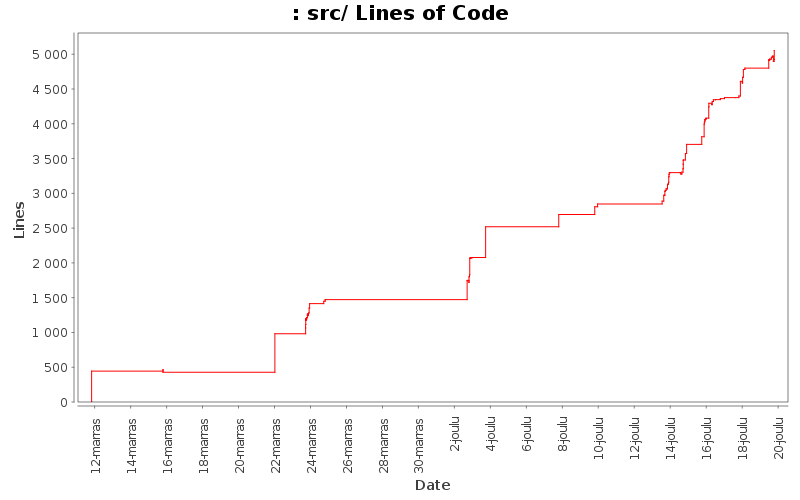
\includegraphics[width=0.6\textwidth]{loc.png}
\caption{The failure to stay within the schedule: lines of code in the src/ directory over time.}
\label{fig:failure}
\end{figure}


\section{Differences to the original plan}
\label{sec-6}

The schedule in the original plan ended up being somewhat a work of
fiction. This was mostly due to the fact that other projects took up
most of the available time.

If the group had had somebody who had designed and/or programmed a
game in detail beforehand, a more detailed plan could have worked
better. Many details were left ambiguous, decisions to be made during
the implementation.

The core features are present:

\begin{itemize}
\item Mouse input with keyboard shortcuts
\item Multiple enemy types with different properties (hit points, speed)
\item Multiple upgradeable tower types: direct, splash and special damage
\item Easy-to-read, easy-to-edit format for maps
\item Towers can be placed at any time
\item Dynamic paths for enemies
\item Multiple terrain types
\item Player profiles, player progress
\end{itemize}

However, as we ran out of time, practically no additional features
were implemented, even though a few of them would have been
easy. Instead, some time was taken to polish the details and to do
additional testing. Multiple entry points and scrollable maps were
implemented. Automatic testing was not included in the build process;
in retrospect several bugs could have been avoided by having a proper
testing procedure. Some parts of the code were implemented using tests
implemented with the Boost test library, but no large scale testing
was done.

\section{References}
\label{sec-7}

\begin{itemize}
\item \href{http://www.cplusplus.com}{C++ documentation}
\item \href{http://www.clanlib.org}{Clanlib documentation}
\end{itemize}

\end{document}